\documentclass[aspectratio=169]{beamer}
\usepackage{etex} % fixes new-dimension error
\usepackage{lmodern}
\usepackage[T1]{fontenc}

\usepackage{graphicx,amsmath}
\usepackage{stmaryrd} % cf. interleave
\usepackage{booktabs}
\usepackage{amscd}
\usepackage{multicol}
\usepackage[absolute,overlay]{textpos}
\usepackage{alltt}
\usepackage{proof}
\usepackage{subcaption}
\usepackage{tikz}
\usepackage{tikz-cd}
\usepackage[new]{old-arrows}
\usepackage[all]{xy}
\usepackage{pgfplots}
\usepackage{textcomp}

\usepackage{transparent}
\usepackage{xspace}
\usepackage{listings}
\usepackage{pdfpages}
\usepackage{relsize}



%%%%%%%%%%%%% Macros
% \newcommand{\Ban}{\catfont{Ban}}
% \newcommand{\Cats}{\catfont{Cat}}

%%%% Misc
%% Operations
\newcommand{\sem}[1]{\llbracket #1 \rrbracket}
\DeclareMathOperator{\img}{\mathrm{im}}
\DeclareMathOperator{\dom}{\mathrm{dom}}
\DeclareMathOperator{\codom}{\mathrm{codom}}
%% Sets of numbers
\newcommand{\N}{\mathbb{N}}
\newcommand{\Z}{\mathbb{Z}}
\newcommand{\Nats}{\mathbb{N}}
\newcommand{\Reals}{\mathbb{R}}
\newcommand{\Rz}{\Reals_{\geq 0}}
\newcommand{\Complex}{\mathbb{C}}
%% Writing
\newcommand{\cf}{\emph{cf.}}
\newcommand{\ie}{\emph{i.e.}}
\newcommand{\eg}{\emph{e.g.}}
\newcommand{\df}[1]{\emph{\textbf{#1}}}
%%%%%%%%%%%%%%%% End of Misc

%%%% Programming Stuff
%% Types
\newcommand{\typefont}[1]{\mathbb{#1}}
\newcommand{\typeOne}{1}
\newcommand{\typeTwo}{2}
\newcommand{\typeA}{\typefont{A}}
\newcommand{\typeX}{\typefont{X}}
\newcommand{\typeB}{\typefont{B}}
\newcommand{\typeC}{\typefont{C}}
\newcommand{\typeV}{\typefont{V}}
\newcommand{\typeD}{\typefont{D}}
\newcommand{\typeI}{\typefont{I}}
%% RuleName
\newcommand{\rulename}[1]{(\mathrm{#1})}
%% Sequents
\newcommand{\jud}{\vdash}
\newcommand{\vljud}{\rhd}
\newcommand{\cojud}{\vdash_{\co}}
\newcommand{\vl}{\mathtt{v}}
\newcommand{\co}{\mathtt{c}}
% Program font
\newcommand{\prog}[1]{\mathtt{#1}}
\newcommand{\pseq}[3]{#1 \leftarrow #2; #3}
\newcommand{\ppm}[4]{(#1,#2) \leftarrow #3; #4}
\newcommand{\pinl}[1]{\prog{inl}(#1)}
\newcommand{\pinr}[1]{\prog{inr}(#1)}
\newcommand{\pcase}[4]{\prog{ case } #1 \prog{ of } \pinl{#2} \Rightarrow #3 ; \pinr{#2} \Rightarrow #4}
%% Sets of terms
\newcommand{\ValuesBP}[2]{\mathsf{Values}(#1, #2)}
\newcommand{\TermsBP}[2]{\mathsf{Terms}(#1, #2)}
\newcommand{\closValP}[1]{\ValuesBP{\emptyset}{#1}}
\newcommand{\closTermP}[1]{\TermsBP{\emptyset}{#1}}
\newcommand{\closVal}{\closValP{\typeA}}
\newcommand{\closTerm}{\closTermP{\typeA}}
%% Contextual equivalence
\newcommand{\ctxeq}{\equiv_{\prog{ctx}}}
%%%% End of Programming Stuff


% Misc by José
\newcommand{\wrap}[2][]{\begin{tabular}[#1]{@{}c@{}}#2\end{tabular}}
\newcommand{\mwrap}[1]{\ensuremath{\begin{array}{@{}c@{}}#1\end{array}}}
\def\trans#1{\xrightarrow{#1}}  % - a - > 
\def\Trans#1{\stackrel{#1}{\Longrightarrow}} % =a=> 
\newcommand{\transp}[2][35]{\color{fg!#1}#2}
\newcommand{\transpt}[2][.35]{\tikz{\node[inner sep=1pt,fill opacity=0.5]{#2}}}
\newcommand{\faded}[2][0.4]{{\transparent{#1}#2}} % alternative to "transp" using transparent package
\newcommand{\set}[1]{\left\{ #1 \right\}} % {a,b,...z}
\newcommand{\mi}[1]{\ensuremath{\mathit{#1}}\xspace}
\newcommand{\mf}[1]{\ensuremath{\mathsf{#1}}\xspace}
% \newcommand{\gold}[1]{\textcolor{darkgoldenrod}{#1}\xspace}


%------ using color ---------------------------------------------------------
\definecolor{goldenrod}{rgb}{.80392 .60784 .11373}
\definecolor{darkgoldenrod}{rgb}{.5451 .39608 .03137}
\definecolor{brown}{rgb}{.15 .15 .15}
\definecolor{darkolivegreen}{rgb}{.33333 .41961 .18431}
\definecolor{myGray}{gray}{0.85}
%
%
\newcommand{\red}[1]{\textcolor{red!80!black}{#1}\xspace}
\newcommand{\blue}[1]{\textcolor{blue}{#1}\xspace}
\newcommand{\gold}[1]{\textcolor{darkgoldenrod}{#1}\xspace}
\newcommand{\gray}[1]{\textcolor{myGray}{#1}\xspace}
% \def\alert#1{{\darkgoldenrod #1}}
% \def\alert#1{{\alert{#1}}}
%\def\brw#1{{\brown #1}}
% \def\structure#1{{\blue #1}}
% \def\tstructure#1{\textbf{\darkblue #1}}
%%\def\gre#1{{\green #1}}
\def\gre#1{{\darkolivegreen #1}}
\def\gry#1{{\textcolor{gray}{#1}}}
\def\rdb#1{{\red #1}}
\def\st{\mathbf{.}\,}
\def\laplace#1#2{*\txt{\mbox{ \fcolorbox{black}{myGray}{$\begin{array}{c}\mbox{#1}\\\\#2\\\\\end{array}$} }}}
%\newcommand{\galois}[2]{#1\; \dashv\; #2}



\def\ainv#1{\overline{#1}}
\def\aconv#1{#1^{\circ}} 
\def\rtran#1{\stackrel{#1}{\longrightarrow}}
\def\pair#1{\langle #1 \rangle}
\def\setdef#1#2{\mathopen{\{} #1 \asor #2 \mathclose{\}}}
\def\imp{\mathbin{\Rightarrow}}
\def\dimp{\mathbin{\Leftrightarrow}}
\def\rimp{\mathbin{\Leftarrow}}
\def\rra{\longrightarrow}
% \def\rcb#1#2#3#4{\def\nothing{}\def\range{#3}\mathopen{\langle}#1 \ #2 \ \ifx\range\nothing::\else: \ #3 :\fi \ #4\mathclose{\rangle}}
\def\abv{\stackrel{\rm abv}{=}}



% Spliting frames in 2 columns
\newcommand{\splittwo}[4]{ 
  \begin{columns}[T]% align columns
  \begin{column}{#1\textwidth} #3 \end{column} ~~~
  \begin{column}{#2\textwidth} #4 \end{column} \end{columns}
}\newcommand{\frsplit}[3][.48]{
  \begin{columns}%[T] % align columns
  \begin{column}{#1\textwidth} #2 \end{column} ~~~
  \begin{column}{#1\textwidth} #3 \end{column} \end{columns}
}
\newcommand{\frsplitdiff}[5][]{
  \begin{columns}[#1]%[T] % align columns
  \begin{column}{#2\textwidth} #4 \end{column} ~~~
  \begin{column}{#3\textwidth} #5 \end{column} \end{columns}
}
\newcommand{\frsplitt}[3][.48]{
  \begin{columns}[T] % align columns
  \begin{column}{#1\textwidth} #2 \end{column} ~~~
  \begin{column}{#1\textwidth} #3 \end{column} \end{columns}
}
\newcommand{\col}[2][.48]{\begin{column}{#1\textwidth} #2 \end{column}}
\newcommand{\colb}[3][.48]{\begin{column}{#1\textwidth} \begin{block}{#2} #3 \end{block} \end{column}}

% Spliting frames in 3 columns
\newcommand{\splitthree}[6]{
  \begin{columns}[T] % align columns
  \begin{column}{#1\textwidth} #4 \end{column} ~~~
  \begin{column}{#2\textwidth} #5 \end{column} ~~~
  \begin{column}{#3\textwidth} #6 \end{column} \end{columns}
}
\newcommand{\frsplitthree}[4][.31]{
  \begin{columns}%[T] % align columns
  \begin{column}{#1\textwidth} #2 \end{column} ~~~
  \begin{column}{#1\textwidth} #3 \end{column} ~~~
  \begin{column}{#1\textwidth} #4 \end{column} \end{columns}
}
\newcommand{\frsplitdiffthree}[7][]{
  \begin{columns}[#1]%[T] % align columns
  \begin{column}{#2\textwidth} #5 \end{column} ~~~
  \begin{column}{#3\textwidth} #6 \end{column} ~~~
  \begin{column}{#4\textwidth} #7 \end{column} \end{columns}
}
\newcommand{\frsplittthree}[4][.32]{
  \begin{columns}[T] % align columns
  \begin{column}{#1\textwidth} #2 \end{column} ~
  \begin{column}{#1\textwidth} #3 \end{column} ~
  \begin{column}{#1\textwidth} #4 \end{column} \end{columns}
}


\newcommand{\typerule}[4][]{\ensuremath{\begin{array}[#1]{c}\textsf{\scriptsize ({#2})} \\#3 \\\hline\raisebox{-3pt}{\ensuremath{#4}}\end{array}}}
\newcommand{\styperule}[3][]{\ensuremath{\begin{array}[#1]{c} #2 \\[0.5mm]\hline\raisebox{-4pt}{\ensuremath{#3}}\end{array}}}
\newcommand{\shrk}{\vspace{-3mm}}

\def\caixa#1{\medskip
  \begin{center}
  \fbox{\begin{minipage}{0.9\textwidth}\protect{#1}\end{minipage}}
  \end{center}}

\newcommand{\mybox}[2][4mm]{
  % \begin{minipage}{#1\textwidth}\begin{block}{}\centering #2\end{block}\end{minipage}}
  \tikz{\node[fill=barcolor!60,align=center,inner sep=#1]{#2};}}
\newcommand{\mycbox}[2][4mm]{
  \begin{center}\mybox[#1]{#2}\end{center}}
  % {\\[-5mm]\centering\mybox[#1]{#2}\\[-5mm]}}

%%%%% Tikz
% \usetikzlibrary{arrows.meta, calc, fit, tikzmark}
\usetikzlibrary{%
  positioning
 ,patterns
 ,arrows
 ,arrows.meta
 ,automata
 ,calc
 ,shapes
 ,fit
 ,tikzmark
 ,fadings
 ,decorations.pathreplacing
 ,plotmarks
% ,pgfplots.groupplots
 ,decorations.markings
 ,shadows
}
% \tikzset{shorten >=1pt,node distance=2cm,on grid,auto,initial text={},inner sep=2pt}
\tikzstyle{aut}=[shorten >=1pt,node distance=2cm,on grid,auto,initial text={},inner sep=2pt]
\tikzstyle{st}=[circle,draw=black,fill=black!10,inner sep=3pt]
\tikzstyle{sst}=[rectangle,draw=none,fill=none,inner sep=3pt]
\tikzstyle{final}=[accepting]

%%% Uppaal-like diagrams
\newcommand{\uppbox}[3][20mm]{\tikz{
  \node[black!15,fill=black!15,minimum width=#1,align=left](title){\textbf{{\footnotesize #2}}};
  \node[black!15,fill=black!15,left,xshift=4mm]at(title.east){\textbf{{\footnotesize #2}}};
  \node[blue!60!cyan,right] at(title.west){\textbf{{\footnotesize #2}}};
  \node[below,inner sep=2mm,fill=white,xshift=2mm](box)at(title.south){\includegraphics[width=#1]{#3}};
  \node[fit=(title)(box),draw=black,inner sep=0pt]{};
}}

\newcommand{\uppboxv}[3][20mm]{\tikz{
  \node[below,inner sep=2mm,fill=white](box){\includegraphics[height=#1]{#3}};
  \coordinate[yshift=5mm](top)at(box.north);
  \node[fit=(top)(box.north west)(box.north east),inner sep=0pt,fill=black!15](title){};
  \node[blue!60!cyan,right] at(title.west){\textbf{{\footnotesize #2}}};
  \node[fit=(title)(box),draw=black,inner sep=0pt]{};
}}

%%% frame for pictures [graphics-options]{content}
\newcommand{\includegraphicsframed}[2][]{\tikz{
  \node[below,inner sep=1mm,fill=barcolor,%xshift=2mm,
    draw=black,
    drop shadow={
      top color=gray,
      bottom color=white,
      %fill=gray,
      opacity=0.2,
      shadow xshift=4pt,
      shadow yshift=-3pt
    }](box){\includegraphics[#1]{#2}};
}}


%% COnfiguring Listings
\lstset{ % basic style
  language=scala,
  basicstyle=\ttfamily\scriptsize,
  breakatwhitespace=true,
  breaklines=true,
  % mathescape,
  % morecomment=[l]{//},
  % morecomment=[n]{/*}{*/},
  % frame=single,                    % adds a frame around the code
  rulecolor=\color{black!40},         % if not set, the frame-color may be changed on line-breaks within not-black text (e.g. comments (green here))
  xleftmargin=1.5mm,
  xrightmargin=1.5mm,
  backgroundcolor=\color{black!5},
  % line numbers
%  numbers=left,  % where to put the line-numbers; possible values are (none, left, right)
 numbersep=5pt, % how far the line-numbers are from the code
 numberstyle=\tiny\color{gray},   
 stepnumber=1,  % the step between two line-numbers. If it is 1 each line will be numbered      
%  xleftmargin=3mm,
%  xrightmargin=1.5mm,
%%%%%
  captionpos=b, % t or b (top or bottom)
  belowcaptionskip=5mm,
%%%%%
  % alsoletter={-},
  % emphstyle=\ttfamily\color{blue}, %\underbar,
  % emphstyle={[2]\ttfamily\color{green!50!black}},
  emphstyle=\bfseries\itshape\color{blue!80!black},       % moreemph={...} - layer keywords
  emphstyle={[2]\itshape\color{red!70!black}},%\underbar} % moreemph={[2]...} - inner keywords
  %
  keywordstyle=\bf\ttfamily\color{red!50!black},
  commentstyle=\sl\ttfamily\color{gray!70},
  % commentstyle=\color{green!60!black},
  stringstyle=\ttfamily\color{green!60!black},
  morestring=[b]",
  % morecomment=[l]{\#},
  frame=single,
  % numberstyle=\tiny, numbers=left, stepnumber=1, firstnumber=1, numberfirstline=true,
  %emph={act,proc,init,sort,map,var,eqn},
  %emph={[2]block,hide,comm,rename,allow,||,<>,sum,&&,=>,true,false},
  literate={\\§}{{{\mbox{\textdollar}}}}1,
  % literate=*{->}{{{\color{red!70!black}$\to$}}}{1}
  %            {.}{{{\color{red!70!black}.}}}{1}
  %            {+}{{{\color{red!70!black}\hspace*{1pt}+\hspace*{1pt}}}}{1}
  %            {|}{{{\color{red!70!black}|}}}{1}
  %            {||}{{{\color{red!70!black}|\!\!|}}}{1}
  %            {*}{{{\color{red!70!black}*}}}{1}
  %            {\#}{{{\color{red!70!black}\#}}}{1}
  %            {&}{{{\color{red!70!black}\&}}}{1}
  %            {:=}{{{\color{red!70!black}:=}}}{1}
  %            {=>}{{{\color{red!70!black}=>}}}{1}
  %            % {>}{{{\color{green!65!black}\hspace*{1pt}>\hspace*{1.5pt}}}}{2}
  %            % {<}{{{\color{green!65!black}\hspace*{1.5pt}<\hspace*{1pt}}}}{2}
  %            % {]}{{{\color{green!65!black}\hspace*{1pt}]\hspace*{1.5pt}}}}{1}
  %            % {[}{{{\color{green!65!black}\hspace*{1.5pt}[\hspace*{1pt}}}}{1}
  %            {>}{{{\color{green!65!black}>}}}{1}
  %            {<}{{{\color{green!65!black}<}}}{1}
  %            {]}{{{\color{green!65!black}]}}}{1}
  %            {[}{{{\color{green!65!black}[}}}{1}
  %  morekeywords={Merger1,Fifo2,Lossy3,Init1,Init2}
  % ,emph={act,proc,init,sort,map,var,eqn}
  % ,emph={[2]block,hide,comm,rename,allow,||,<>,sum,&&,=>}
}

\newcommand{\code}[1]{{\relsize{-1}\ttfamily #1}}
\newcommand{\cod}[1]{{\relsize{-0.5}\color{blue!75!black}\ttfamily #1}}
% \definecolor{mydarkgreen}{rgb}{0,0.6,0}
% \newcommand{\bash}[1]{\lstinline[basicstyle=\ttfamily\relsize{-0.5}\color{mydarkgreen},keywordstyle=\bf\sffamily\color{purple},columns=fullflexible,keepspaces,literate=*]|#1|}

\lstdefinestyle{tiny}{basicstyle=\ttfamily\relsize{-7}}

% Include slides from others
\newcommand{\byothers}[3]{{
\begin{frame}{}~\mycbox{\Large slides by #1\\pages #2}\end{frame}{}
\setbeamercolor{background canvas}{bg=}
\includepdf[pages=#2]{../../others/#3}
}}

\newcounter{mypage}
\newcommand{\fromBook}[6][scale=0.5]{
\setcounter{mypage}{20}
\addtocounter{mypage}{#2}
\begin{tabular}{@{}r@{}}
\includegraphics[page=\themypage, trim = #3 #4 #5 #6, clip, #1]%
  {../../learning-concurrent-scala/learning-concurrent-programming-in-scala.pdf}
  \\[0mm]
  \textcolor{myGray}{$\left[\begin{array}{@{}r@{}}
  ~\\[-7mm]
  \text{{\tiny in \emph{``Learning Concurrent}}}\\[-3mm]
  \text{{\tiny \emph{Programming in Scala''}, pg.\,#2}}
  \\[0mm]
  \end{array}\right]$}
\end{tabular}
}

\newcommand{\fromBookW}[4][width=\textwidth]{
\setcounter{mypage}{20}
\addtocounter{mypage}{#2}
\begin{tabular}{@{}r@{}}
\includegraphics[page=\themypage, trim = 20mm #3 20mm #4, clip, #1]%
  {../../learning-concurrent-scala/learning-concurrent-programming-in-scala.pdf}
  \\[-2mm]
  \textcolor{myGray}{$\left[\begin{array}{@{}r@{}}
  ~\\[-7mm]
  \text{{\tiny in \emph{``Learning Concurrent}
                      \emph{Programming in Scala''}, pg.\,#2}}
  \\[0mm]
  \end{array}\right]$}
\end{tabular}
}

\newcommand{\fromBookWframed}[4][width=\textwidth]{
\setcounter{mypage}{20}
\addtocounter{mypage}{#2}
\begin{tabular}{@{}r@{}}
\includegraphicsframed[page=\themypage, trim = 20mm #3 20mm #4, clip, #1]%
  {../../learning-concurrent-scala/learning-concurrent-programming-in-scala.pdf}
  \\[-2mm]
  \textcolor{myGray}{$\left[\begin{array}{@{}r@{}}
  ~\\[-7mm]
  \text{{\tiny in \emph{``Learning Concurrent}
                      \emph{Programming in Scala''}, pg.\,#2}}
  \\[0mm]
  \end{array}\right]$}
\end{tabular}
}

\newcommand{\fromAuthor}[3][width=\textwidth]{
\begin{tabular}{@{}r@{}}
\includegraphics[#1]%
  {src/img/#3}
  \\[-2mm]
  \textcolor{myGray}{$\left[\begin{array}{@{}r@{}}
  ~\\[-7mm]
  \text{{\tiny in #2}}
  \\[0mm]
  \end{array}\right]$}
\end{tabular}
}


%-------------- template --------------------------------------------------
 %!TEX root=../../1-intro.tex
 \usetheme{metropolis}
\usepackage{appendixnumberbeamer}

%------ Setting lecture info ----------------------------------------------
\newcounter{lectureID}
\stepcounter{lectureID}
\newcommand{\getLecture}{\arabic{lectureID}\xspace}
\newcommand{\setLectureBasic}[1]{
  \title{
    #1
    }
  \author{Nelma Moreira ~~\&~~ \textbf{Jos\'{e} Proen\c{c}a}}
  \institute{CISTER -- U.Porto, Porto, Portugal
            \hfill 
            \begin{tabular}{r@{}}
            \url{https://fm-dcc.github.io/cp2425}
            \end{tabular}
            }
  \date{Concurrent programming (CC3040) 2024/2025}
  % logos of institutions
  \titlegraphic{
    \begin{textblock*}{5cm}(2.0cm,7.00cm)
       
\includegraphics[scale=0.14]{src/img/logos/fcup}\hspace*{.85cm}~%
    \end{textblock*}
    \begin{textblock*}{5cm}(6.0cm,7.25cm)
      
\includegraphics[scale=0.43]{src/img/logos/cmup}
    \end{textblock*}
    \begin{textblock*}{5cm}(10.4cm,7.45cm)
      
\includegraphics[scale=0.16]{src/img/logos/cister}
    \end{textblock*}
  }  
  \frame[plain]{\titlepage}
}
\newcommand{\setLecture}[2]{\setcounter{lectureID}{#1}\setLectureBasic{#1. #2}}

%------ Counters for exercises ----------------------------------------------
\newcounter{cExercise}
\newcommand{\exercise}{\stepcounter{cExercise}Ex.\,\arabic{lectureID}.\arabic{cExercise}:\xspace}
\newcommand{\exerciseBack}{\addtocounter{cExercise}{-1}}
\newcommand{\exerciseAdd}{\stepcounter{cExercise}}
\newcommand{\doExercise}[3][0mm]{\begin{exampleblock}{\exercise #2}\wrap{\rule{0pt}{#1}}#3\end{exampleblock}}
\newcommand{\doSimpleExercise}[2][0mm]{\begin{exampleblock}{}\wrap{\rule{0pt}{#1}}\structure{\textbf{\exercise} #2}\end{exampleblock}}

% Slide
\newenvironment{slide}[1]{\begin{frame}\frametitle{#1}}{\end{frame}}



% Base colors (from metropolis theme)
\definecolor{metDarkBrown}{HTML}{604c38}
\definecolor{metDarkTeal}{HTML}{23373b}
\definecolor{metLightBrown}{HTML}{EB811B}
\definecolor{metLightGreen}{HTML}{14B03D}
\definecolor{metDarkGreen}{HTML}{4f9277}

 

\metroset{numbering=fraction,progressbar=frametitle}

% \setbeamercolor*{structure}{fg=blue!80!black}
\setbeamercolor*{structure}{fg=metLightGreen}

% % \definecolor{MainColour}{rgb}{0., 0.25, 0.8}
% \colorlet{MainColour}{blue!50!black}
% \colorlet{BgColour}{blue!10}
% \colorlet{BarColour}{blue!50!black}

% %\usetheme{CambridgeUS}%{Copenhagen}%{Frankfurt}%{Singapore}%{CambridgeUS}
% \usecolortheme[named=MainColour]{structure} 
% \useoutertheme[subsection=false]{miniframes}
% \useinnertheme{circles}
% %\useinnertheme[shadow=false]{rounded}
% \setbeamertemplate{blocks}[rounded][shadow=false]

% \setbeamercovered{transparent} 
% \setbeamertemplate{navigation symbols}{} %Remove navigation bar
% \setbeamertemplate{footline}[frame number] % add page number
% \setbeamercolor{postit}{fg=MainColour,bg=BgColour}
% \setbeamercolor{structure}{bg=black!10}
% %\setbeamercolor{palette primary}{use=structure,fg=red,bg=green}
% %\setbeamercolor{palette secondary}{use=structure,fg=red!75!black,bg=green}
% \setbeamercolor{palette tertiary}{use=structure,bg=BarColour,fg=white}
% %\setbeamercolor{palette quaternary}{fg=black,bg=green}
% %\setbeamercolor{normal text}{fg=black,bg=white}
% %\setbeamercolor{block title alerted}{fg=red,bg=green}
% %\setbeamercolor{block title example}{bg=black!10,fg=green}
\setbeamercolor{block body}{bg=black!5}

% \setbeamercolor{block title alerted}{bg=red!25}
% \setbeamercolor{block body alerted}{bg=red!10}

% \setbeamercolor{block title example}{bg={rgb:green,2;black,1;white,5}}
\setbeamercolor{block body example}{bg={rgb:green,2;black,1;white,20}}
\setbeamercolor{block body alerted}{bg={metLightBrown!25}}

% \setbeamertemplate{itemize item}{\color{black!10}$\blacksquare$}
\setbeamercolor{itemize item}{fg=metDarkTeal}
\setbeamercolor{itemize subitem}{fg=metDarkTeal}

\setbeamercolor{graybc}{fg=black,bg=black!10}
\newcommand{\myblock}[1]{\begin{beamercolorbox}[dp=1ex,center,rounded=true]%
  {graybc} {\large \textbf{#1}} \end{beamercolorbox}}%

%%%%%%%%%

% \definecolor{barcolor}{rgb}{.65,.79,.92} % FCUP color
\colorlet{barcolor}{metDarkGreen!60}


% Configuring the foot line
\setbeamercolor{author in head/foot}{fg=metDarkTeal, bg=barcolor}%
\setbeamercolor{date in head/foot}{fg=barcolor!75!black}%
\setbeamertemplate{footline}
{
  \leavevmode%
  \hbox{%
  \begin{beamercolorbox}[wd=.4\paperwidth,ht=2.25ex,dp=1ex,center]{author in head/foot}%
    \usebeamerfont{author in head/foot}\insertshortauthor
  \end{beamercolorbox}%
  \begin{beamercolorbox}[wd=.5\paperwidth,ht=2.25ex,dp=1ex,center]{title in head/foot}%
    \usebeamerfont{title in head/foot}\insertsection
  \end{beamercolorbox}%
  \begin{beamercolorbox}[wd=.1\paperwidth,ht=2.25ex,dp=1ex,right]{date in head/foot}%
    \insertframenumber{} / \inserttotalframenumber\hspace*{2ex} 
  \end{beamercolorbox}}%
  \vskip0pt%
}
% No configuration symbols
\setbeamertemplate{navigation symbols}{}


%%%%%%% Custom bar above

\setbeamercolor{frametitle}{bg=barcolor,fg=metDarkTeal}
\setbeamercolor{progress bar}{fg=barcolor!75!black}

%%% Custom bar with a LOGO

\makeatletter
\setbeamertemplate{frametitle}{%
  \nointerlineskip%
  \begin{beamercolorbox}[%
      wd=\paperwidth,%
      sep=0pt,%
      leftskip=\metropolis@frametitle@padding,%
      rightskip=\metropolis@frametitle@padding,%
    ]{frametitle}%
  \metropolis@frametitlestrut@start%
  \insertframetitle%
  \nolinebreak%
  \metropolis@frametitlestrut@end%
  \hfill
  \raisebox{-1.3ex}{
\includegraphics[height=4ex,keepaspectratio]{src/img/logos/fcup-bar}}
  \end{beamercolorbox}%
}
\makeatother





%----------------------------------------------------------------------------

\begin{document}

\setLecture{3}{Concurrency in Java and its memory model}


\section{Overview}

\begin{frame}{We are here}

  \vspace*{-2mm}

  \begin{block}{Blocks of sequential code running concurrently and sharing memory:}
    
  \begin{itemize}
    \item What is Scala?
    \alert{\item Concurrency in Java and its memory model}
    \item Basic concurrency blocks and libraries
    \item \textcolor{gray}{Futures and promises}
    \item Actor model
  \end{itemize}
  \end{block}
\end{frame}


\begin{frame}\frametitle{Traditional concurrency}
  \splittwo{0.49}{0.49}{
  \begin{block}{Synchronisation}
    - Coordination of multiple executions in a concurrent system
    \\- Mechanisms to \structure{order} concurrent executions
    \\- Mechanisms to \structure{exchange} information
  \end{block}
  }{
  \begin{block}{Exchanging information}
    - \alert{Concurrent programs: shared memory communication}
    \\- Distributed programs: message passing communication
    
  \end{block}
  }
\end{frame}


\begin{frame}\frametitle{Processes and threads}\centering
  \splittwo{0.46}{0.52}{
    % \fromBookW[scale=0.7]{32}{98mm}{39mm}
    \fromBook[scale=0.65]{32}{43mm}{98mm}{43mm}{39mm}
  }{
    ~\\[4mm]
    Starting a new JVM instance always creates \alert{only one} process.
    \\[4mm]
    In that process, \alert{multiple threads} can run simultaneously.
    \\[4mm]
    Unlike runtimes (e.g. Python), the JVM:
    \\~~does not implement its custom threads,
    \\~~maps each \structure{Java thread} to an \structure{OS thread}
  }
\end{frame}


\section{Managing threads}

\begin{frame}[fragile]\frametitle{Current thread}
~\\[-8mm]
\begin{columns}
\begin{column}{0.49\textwidth}
\begin{lstlisting}
object ThreadsMain extends App {
  val t: Thread = Thread.currentThread
  val name = t.getName
  println(s"I am the thread \§name")
}
\end{lstlisting}
\end{column}
\begin{column}{0.49\textwidth}
Using SBT, this prints:
\\\code{[info] I am the thread sbt-bg-threads-1}
\\[4mm]
In SBT do ``\code{set fork := true}''
\\
It will then it prints:
\\\code{[info] I am the thread main}
\end{column}
\end{columns}
\end{frame}


\begin{frame}[fragile]\frametitle{Creating threads}
~\\[-8mm]
\begin{columns}
\begin{column}{0.49\textwidth}
\begin{lstlisting}[emph={start,join,run}]
object ThreadsCreation extends App {
  class MyThread extends Thread {
    override def run(): Unit = {
      println("New thread running.")
    }
  } 
  val t = new MyThread
  t.start()
  t.join()
  println("New thread joined.")
}
\end{lstlisting}
\end{column}
\begin{column}{0.49\textwidth}
\alert{\code{start}} eventually causes
\\\alert{\code{run}} to execute in a new thread;
\\[4mm]
the OS decides when;
\\[4mm]
\alert{\code{join}} puts the main thread in a \structure{waiting state}, and allows the OS to re-assign the processor.
% \\[4mm]
\end{column}
\end{columns}
\end{frame}

\begin{frame}%\frametitle{title}
  \fromBookW{35}{32mm}{126mm}
\end{frame}


\begin{frame}[fragile]\frametitle{Simpler thread creation}
~\\[-8mm]
\begin{columns}
\begin{column}{0.49\textwidth}
\begin{lstlisting}[emph={thread,run,start}]
def thread(body: =>Unit): Thread = {
  val t = new Thread {
    override def run() = body
  }
  t.start()
  t
}
\end{lstlisting}
\end{column}
\begin{column}{0.49\textwidth}
\pause
\structure{Using the \code{thread} function}
\begin{lstlisting}[emph={sleep,log,thread,join}]
object ThreadsSleep extends App {
  val t = thread {
    Thread.sleep(1000)
    log("New thread running.")
    Thread.sleep(1000)
    log("Still running.")
    Thread.sleep(1000)
    log("Completed.")
  }
  t.join()
  log("New thread joined.")
}
\end{lstlisting}
\end{column}
\end{columns}
\end{frame}


\begin{frame}%\frametitle{Life-cycle of a thread}
  \centering
  % 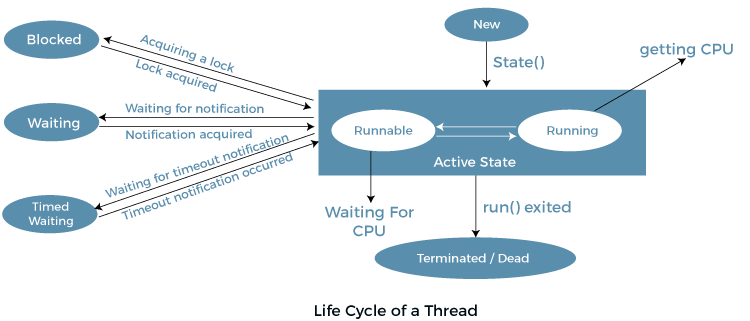
\includegraphics[width=1\textwidth]{src/img/life-cycle-of-a-thread.png}
  % \fromAuthor[width=\textwidth]{https://seeandselect.com/popedaze/life-cycle-of-a-thread}{life-cycle-of-a-thread.png}
  \fromAuthor[width=\textwidth]{https://static.javatpoint.com/core/images/life-cycle-of-a-thread.png}{life-cycle-of-a-thread.png}
\end{frame}

\begin{frame}[fragile]\frametitle{Nondeterministic thread execution}
~\\[-8mm]
\begin{columns}
\begin{column}{0.49\textwidth}
\begin{itemize}
  \item \texttt{``New thread''} printed always at the end
  \item Other prints not always in the same order -- nondeterministic execution
  \item Common in concurrent applications -- what makes it so hard
  \item Note: \texttt{join} also forces all memory writes from the threads before proceeding
\end{itemize}

\end{column}
\begin{column}{0.49\textwidth}
\begin{lstlisting}[emph={sleep,log,thread,join}]
object ThreadsNondeterminism extends App {
  val t = thread {
    log("New thread running.")
  }
  log("...")
  log("...")
  t.join()
  log("New thread joined.")
}
\end{lstlisting}
\end{column}
\end{columns}
\end{frame}


\section{Control of the execution order}

\begin{frame}\frametitle{Happens-before relation}
\centering

\structure{action $\alpha$} \alert{happens-before (HB)} \structure{action $\beta$}\\
means  \structure{action $\beta$} sees the memory writes of \structure{action $\alpha$}

\begin{itemize}
\item \textbf{Program order:} $\alpha$ in a thread \alert{HB} every subsequent $\beta$ in that program and thread
\item \textbf{Thread start:} calling \texttt{thrd.start()} \alert{HB} any actions of \texttt{thrd}
\item \textbf{Thread termination:} $\alpha$ in a thread \alert{HB} a \texttt{join()} on that thread.
\item \textbf{Transitivity:} if $\alpha$ \alert{HB} $\beta$ and $\beta$ \alert{HB} $\gamma$, then $\alpha$ \alert{HB} $\gamma$
\item ...
\end{itemize}

\pause
\structure{Data race:} when a write to memory does not \alert{happen-before} its \emph{intended} read.
\end{frame}



\begin{frame}[fragile]\frametitle{Atomic Execution}
\begin{itemize}
  \item \texttt{join} provides guarantees that other threads terminated
  \item Not enough -- we may want to inform other treads without terminating
\end{itemize}

\textbf{Example 1: shared counter for unique IDs}
\begin{lstlisting}[emph={sleep,log,thread,join}]
object ThreadsUnprotectedUid extends App {
  var uidCount = 0L
  def getUniqueId() = {
    val freshUid = uidCount + 1
    uidCount = freshUid
    freshUid
}
\end{lstlisting}

\structure{What can go wrong?}
\end{frame}


\begin{frame}[fragile]\frametitle{Atomic Execution}
~\\[-8mm]
\begin{columns}
\begin{column}{0.49\textwidth}
\begin{lstlisting}[emph={printUniqueIds,sleep,log,thread,join}]
...
def printUniqueIds(n: Int): Unit = {
  val uids = for (i<- 0 until n) yield getUniqueId()
  log(s"Generated uids: \§uids")
}
val t = thread { printUniqueIds(5) }
printUniqueIds(5)
t.join()
...
\end{lstlisting}
\end{column}
\begin{column}{0.49\textwidth}
\begin{lstlisting}[emph={sleep,log,thread,join}]
object ThreadsNondeterminism extends App {
  val t = thread {
    log("New thread running.")
  }
  log("...")
  log("...")
  t.join()
  log("New thread joined.")
}
\end{lstlisting}
\end{column}
\end{columns}
\only<1>{\structure{What do you expect?}}%
\only<2>{\begin{block}{Race Condition}
  when the \structure{output of a concurrent program} depends on \alert{how the statements are scheduled}.
\end{block}}
\end{frame}

\begin{frame}\frametitle{Updating counter in parallel}
  \centering
  \code{val freshUid = uidCount +  1 ;  uidCount = freshUid  ;  freshUid}

  \medskip
  
  \fromBookW{40}{26mm}{151mm}
\end{frame}

\begin{frame}[fragile]\frametitle{``Synchronized'' to the rescue}
~\\[-8mm]
\begin{columns}
\begin{column}{0.49\textwidth}
\begin{lstlisting}[emph={printUniqueIds,sleep,log,thread,join}]
def getUniqueId() =
   this.synchronized {
      val freshUid = uidCount + 1
      uidCount = freshUid
      freshUid
}
\end{lstlisting}
\end{column}
\begin{column}{0.49\textwidth}
\texttt{synchronized} is:
\begin{itemize}
  \item a fundamental Scala/Java construct for atomic executions
  \item can be called in \structure{any object} (or instance of a class)
  \item ensures atomic execution wrt the object
  \item we say \code{obj.synchronized}
    \begin{itemize}
      \item \alert{acquires} the \structure{lock/monitor} of \structure{obj} at the start
      \item \alert{releases} the \structure{lock/monitor} of \structure{obj} at the end
    \end{itemize}
\end{itemize}
\end{column}
\end{columns}
\end{frame}


\begin{frame}\frametitle{Updating counter in parallel atomically}
  \centering  
  \fromBookW{41}{26mm}{135mm}
\end{frame}

\begin{frame}%\frametitle{Life-cycle of a thread}
  \centering
  \fromAuthor[width=\textwidth]{https://static.javatpoint.com/core/images/life-cycle-of-a-thread.png}{life-cycle-of-a-thread.png}
\end{frame}


\begin{frame}\frametitle{Reordering}
\centering
\begin{itemize}
  \item using the \texttt{synchronized} statement has some (not too large) overhead
  \item not using \texttt{synchronized} can easily lead to errors, even if all seems correct
\end{itemize}

{\large \structure{Find the bug in the next slide...}}
\end{frame}


\begin{frame}[fragile]\frametitle{Find the bug}\label{slide:ThreadSharedStateAccessReordering}
\begin{lstlisting}[emph={assert,sleep,log,thread,join}]
object ThreadSharedStateAccessReordering extends App {
  for (i <- 0 until 100000) {
    var a = false
    var b = false
    var x = -1
    var y = -1
    val t1 = thread {
      a = true
      y = if (b) 0 else 1
    }
    val t2 = thread {
      b = true
      x = if (a) 0 else 1
    }
    t1.join()
    t2.join()
    assert(!(x==1 && y==1), s"x=\§x, y=\§y")
  }
}
\end{lstlisting}
\end{frame}


\begin{frame}\frametitle{Reordering within threads}
\begin{itemize}
  \item The previous code can raise an error: both \texttt{x} and \texttt{y} can become 1!

  \item JVM can reorder statements in a thread when they seem to be independent.

  \item Because some processors do not always execute instructions in the expected order, to increase performance.
  \item (Known as ``weak memory model'')
  \item A \texttt{synchronized} block would solve this:
    \begin{itemize}
      \item also enclosing each assignment in a \texttt{synchronized} block
      \item \texttt{synchronized} sets up a \emph{memory barrier} 
    \end{itemize}
\end{itemize}
\end{frame}




\begin{frame}[fragile]\frametitle{Locks and synchronization}
\begin{itemize}
  \item every object has a \emph{lock}
  \item a running \alert{thread} can \structure{aquire} multiple locks from different objects
\end{itemize}

\textbf{Example 2: Logging Bank Transfers}
\begin{lstlisting}[emph={assert,sleep,log,thread,join,synchronized}]
object SynchronizedNesting extends App {
   import scala.collection._
   
   private val transfers = mutable.ArrayBuffer[String]()
   def logTransfer(name: String, n: Int) = transfers.synchronized {
     transfers += s"transfer to account '\§name' = \§n"
   }
   class Account(val name: String, var money: Int)
   def add(account: Account, n: Int) = account.synchronized {
       account.money += n
       if (n > 10) logTransfer(account.name, n)
   }
   ...
}
\end{lstlisting}
\end{frame}


\begin{frame}[fragile]\frametitle{Locks and synchronization}
\begin{lstlisting}[emph={assert,sleep,log,thread,join,synchronized}]
   private val transfers = mutable.ArrayBuffer[String]()
   def logTransfer(name: String, n: Int) = transfers.synchronized {
     transfers += s"transfer to account '\§name' = \§n"
   }
   class Account(val name: String, var money: Int)
   def add(account: Account, n: Int) = account.synchronized {
       account.money += n
       if (n > 10) logTransfer(account.name, n)
   }

   val jane = new Account("Jane", 100)
   val john = new Account("John", 200)
   val t1 = thread { add(jane, 5) }
   val t2 = thread { add(john, 50) }
   val t3 = thread { add(jane, 70) } // will not corrupt Jane's account
   t1.join(); t2.join(); t3.join()
   log(s"--- transfers ---\n\§transfers")
\end{lstlisting}
\end{frame}


\begin{frame}\frametitle{Happens-before relation (again)}
\centering

\structure{action $\alpha$} \alert{happens-before (HB)} \structure{action $\beta$}\\
means  \structure{action $\beta$} sees the memory writes of \structure{action $\alpha$}

\begin{itemize}
\item \textbf{Program order:} $\alpha$ in a thread \alert{HB} every subsequent $\beta$ in that program and thread
\item \textbf{Thread start:} calling \texttt{thrd.start()} \alert{HB} any actions of \texttt{thrd}
\item \textbf{Thread termination:} $\alpha$ in a thread \alert{HB} a \texttt{join()} on that thread.
\item \textbf{Transitivity:} if $\alpha$ \alert{HB} $\beta$ and $\beta$ \alert{HB} $\gamma$, then $\alpha$ \alert{HB} $\gamma$
\item ...
\structure{
\item \textbf{Monitor locking:} unlocking \alert{HB} every subsequent locking (of the same lock)
}
\end{itemize}

\end{frame}





\section{Deadlocks}

\begin{frame}[fragile]\frametitle{Deadlocks -- the dark side of locks}

\begin{alertblock}{Deadlock}
  when two or more executions wait for each other before proceeding
\end{alertblock}

\begin{itemize}
  \item Studied in the first module with prof. Nelma Moreira
  % \item \structure{Dining philosophers} is a typical example
  \item Often caused by locks that are not released at the right time
\end{itemize}

\begin{lstlisting}[emph={assert,sleep,log,thread,join,synchronized}]
object SynchronizedDeadlock extends App {
  import SynchronizedNesting.Account
  def send(a: Account, b: Account, n: Int) = a.synchronized {
    b.synchronized {
      a.money -= n
      b.money += n
    }
  }
  ... // can this go wrong?
}
\end{lstlisting}
\end{frame}


\begin{frame}[fragile]\frametitle{Deadlocks -- the dark side of locks}
\begin{lstlisting}[emph={assert,sleep,log,thread,join,synchronized}]
  def send(a: Account, b: Account, n: Int) = a.synchronized {
    b.synchronized {
      a.money -= n
      b.money += n
    }
  }

  val l = new Account("Lucy", 1000)
  val j = new Account("Jim", 2000)
  val t1 = thread { for (i<- 0 until 100) send(l, j, 1) }
  val t2 = thread { for (i<- 0 until 100) send(j, l, 1) }
  t1.join(); t2.join()
  log(s"a = ${a.money}, b = ${b.money}")
\end{lstlisting}

{\Large \pause It works but... \pause \alert{it can deadlock}}
\end{frame}


\begin{frame}[fragile]\frametitle{Possible fix: fix order}

\begin{itemize}
  \item always acquire locks in the same order
  \item need a total order on locks
  \item we can use the getUniqueId (Example 1)
\end{itemize}
    
\begin{lstlisting}[emph={getUniqueId,sleep,log,thread,join,synchronized}]
import SynchronizedProtectedUid.getUniqueId
class Account(val name: String, var money: Int) {
  val uid = getUniqueId()
}
\end{lstlisting}
\pause
\begin{lstlisting}[emph={assert,sleep,log,thread,join,synchronized}]
def send(a1: Account, a2: Account, n: Int) {
  def adjust() {
    a1.money -= n
    a2.money += n
  }
  if (a1.uid < a2.uid)  a1.synchronized{ a2.synchronized{ adjust() }}
  else                  a2.synchronized{ a1.synchronized{ adjust() }}
}
\end{lstlisting}
\end{frame}

\section{Guarded blocks}

\begin{frame}\frametitle{Guarded blocks}
\begin{alertblock}{Guarded block (for us)}
  a \structure{block of code} that \alert{waits for a condition} before running in a thread
\end{alertblock}

\begin{block}{Example 3: Thread pool with a queue of tasks}
  \begin{itemize}
    \item Creating \structure{new threads} in Java is \alert{expensive} and \alert{avoidable}
    \item Usually we re-use threads, by maintaining a set of waiting threads
    \item This set is call a thread pool
      \begin{itemize}
        \item Scala already provides thread pools
        \item We first create our own
      \end{itemize}
  \end{itemize}
\end{block}
\end{frame}


\begin{frame}[fragile]\frametitle{}
~\\[-8mm]
\begin{columns}
\begin{column}{0.65\textwidth}
\begin{lstlisting}[emph={synchronized,printUniqueIds,sleep,log,thread,join}]
 import scala.collection._
 object SynchronizedBadPool extends App {
  // our set of tasks
  private val tasks = mutable.Queue[()=>Unit]()
 
  // our single working thread
  val worker = new Thread {
    def poll(): Option[()=>Unit] = 
      tasks.synchronized {
       if (tasks.nonEmpty) Some(tasks.dequeue())
       else                None
      }
    // keep on trying to run forever!
    override def run() = while (true)
      poll() match {
        case Some(task) => task()
        case None =>
    }
  }
\end{lstlisting}
\end{column}
\begin{column}{0.40\textwidth}
\begin{lstlisting}[mathescape,emph={synchronized,sleep,log,thread,join}]
  // starting the worker as a daemon
  worker.setName("Worker")
  worker.setDaemon(true)
  worker.start()

  def asynchr(body: =>Unit) =
    tasks.synchronized {
      tasks.enqueue(()=>body)
    }

  asynchr{ log("Hello")  }
  asynchr{ log(" world!")}
  Thread.sleep(5000)
}



$~$
\end{lstlisting}
\end{column}
\end{columns}
\end{frame}


\begin{frame}\frametitle{Note on daemon threads}
% \splittwo{
  \begin{alertblock}{Daemon thread}
    \begin{itemize}
      \item not the default
      \item have lower priority
      \item terminated automatically when JVM terminates
      \item in other words, do not prevent the JVM from terminating
      \item (the JVM terminates when `normal' tasks terminate)
    \end{itemize}    
  \end{alertblock}
\end{frame}


\begin{frame}\frametitle{Bad busy-waiting}
    
  \begin{block}{Busy-waiting is bad}
    \begin{itemize}
      \item needlessly uses processor power (and drains the battery)
      \item after executing the previous code the \texttt{worker} will keep on running (unless you set in SBT \code{set fork := true},)
      \item in general, we want the \texttt{worker} to enter a waiting state
    \end{itemize}
    
  \end{block}
\end{frame}

\begin{frame}\frametitle{Avoiding busy-waiting}
\centering

{\Large \alert{synchronized} + \structure{wait} + \structure{notify}}

\begin{itemize}
  \item these are methods that every Java/Scala object has
  \item \structure{wait}:
    \begin{itemize}
      \item needs the lock
      \item puts the thread in a \alert{waiting} state
      \item releases the lock until activation
    \end{itemize}
  \item \structure{notify}:
    \begin{itemize}
      \item needs the lock
      \item \alert{activates} all waiting threads
    \end{itemize}
  \pause
  \item Note that the JVM can decide to call \texttt{wait} on its own -- \alert{spurious wakeups} -- needing to re-enter the \emph{wait}
\end{itemize}
\end{frame}

\begin{frame}[fragile]\frametitle{Wait-notify example}
\begin{lstlisting}[emph={sleep,log,thread,join,wait,notify,synchronized}]
object SynchronizedGuardedBlocks extends App {
  val lock = new AnyRef
  var message: Option[String] = None
  val greeter = thread {
    lock.synchronized {
      while (message == None) lock.wait() // non-busy waiting for a message
      log(message.get)                    // it will eventually log!
    }
  }
  lock.synchronized {
    message = Some("Hello!")
    lock.notify()                    // awakes the (possibly) locked thread
  }
  greeter.join()
}
\end{lstlisting}
\end{frame}


\begin{frame}[fragile]\frametitle{Example 3 -- without busy-waiting}
~\\[-8mm]
\begin{columns}
\begin{column}{0.65\textwidth}
\begin{lstlisting}[emph={printUniqueIds,sleep,log,thread,join,synchronized,wait,notify}]
import scala.collection._
object SynchronizedPool extends App {
  private val tasks = mutable.Queue[()=>Unit]()

  object Worker extends Thread {
    setDaemon(true)
    def poll() = tasks.synchronized {
      while (tasks.isEmpty) tasks.wait()
                         // now using wait
      tasks.dequeue()
    }
    override def run() = while (true) {
      val task = poll()
      task()
    }
  }
\end{lstlisting}
\end{column}
\begin{column}{0.40\textwidth}
\begin{lstlisting}[mathescape,emph={sleep,log,thread,join,synchronized,wait,notify}]
  Worker.start()

  def asynchr(body: =>Unit) =
    tasks.synchronized {
       tasks.enqueue(()=>body)
       // now notifying
       tasks.notify()
    }

  asynchr{ log("Hello")  }
  asynchr{ log(" world!")}
  Thread.sleep(500)
}


$~$
\end{lstlisting}
\end{column}
\end{columns}


\end{frame}



\begin{frame}\frametitle{Interrupting threads -- \texttt{Thread.interrupt()}}
\begin{itemize}
  \item Our \texttt{Worker} can run forever (\texttt{while-true})
  \item Terminates when the JVM terminates (daemon)
  \item \texttt{Worker} can be terminated earlier while waiting
    \begin{itemize}
      \item \alert{\texttt{Worker.interrupt()}}
      \item triggers an \alert{\texttt{InterruptedException}} that can be handled
      \item if it was not waiting, then no exception is raised
      \item instead a flag \alert{\texttt{Worker.isInterrupted}} becomes true
      \item needed if the thread does not awake with \texttt{notify} (e.g., it is doing blocking I/O)
    \end{itemize}
\end{itemize}
\end{frame}

\begin{frame}[fragile]\frametitle{Interrupting threads -- alternative with \alert{graceful shutdown}}
    
\begin{lstlisting}[emph={sleep,log,thread,join,synchronized,wait,notify,shutdown,terminated}]
object Worker extends Thread {
  var terminated = false
  // "manually" terminate when asked
  def poll(): Option[() => Unit] = tasks.synchronized {
    while (tasks.isEmpty && !terminated) tasks.wait()
    if (!terminated) Some(tasks.dequeue()) else None
  }

  import scala.annotation.tailrec
  @tailrec override def run() = poll() match {
    case Some(task) => task(); run()
    case None =>
  }
  // "manually" ask to terminate
  def shutdown() = tasks.synchronized {
    terminated = true
    tasks.notify()
  }
}
\end{lstlisting}

\end{frame}


\begin{frame}\frametitle{Volatile variables -- Alternative to \texttt{lock.synchronized}}
\begin{itemize}
  \item using the \texttt{\alert{@volatile}} annotation
  \\~
  \item can be [atomically read] and [atomically modified]
  \item mostly used as status flag
  \item are never reordered in a thread
  \item writes are immediately visible to other threads
  \item very cheap to read
  \item not enough in many situations (e.g., \texttt{getUniqueID})
  \item enough for previous example -- Slide~\ref{slide:ThreadSharedStateAccessReordering}
\end{itemize}
\end{frame}

\begin{frame}[fragile]\frametitle{Example 4 -- Batman}
\begin{lstlisting}[emph={sleep,log,thread,join,synchronized,wait,notify,volatile,found}]
object Volatile extends App {
  class Page(val txt: String, var position: Int)

  val pages = for (i<- 1 to 5) yield
    new Page("Na" * (100 - 20 * i) + " Batman!", -1)
  @volatile var found = false
  for (p <- pages) yield thread {
    var i = 0
    while (i < p.txt.length && !found)
      if (p.txt(i) == '!') {
        p.position = i
        found = true
      } else i += 1
  }
  while (!found) {}
  log(s"results: \§{pages.map(_.position)}")
}
\end{lstlisting}
\end{frame}


\section{The Java Memory Model overview}

\begin{frame}\frametitle{Happens-before relation}
\centering

\structure{action $\alpha$} \alert{happens-before (HB)} \structure{action $\beta$}\\
means  \structure{action $\beta$} sees the memory writes of \structure{action $\alpha$}

\begin{itemize}
\item \textbf{Program order:} $\alpha$ in a thread \alert{HB} every subsequent $\beta$ in that program and thread
\item \textbf{Thread start:} calling \texttt{thrd.start()} \alert{HB} any actions of \texttt{thrd}
\item \textbf{Thread termination:} $\alpha$ in a thread \alert{HB} a \texttt{join()} on that thread.
\item \textbf{Transitivity:} if $\alpha$ \alert{HB} $\beta$ and $\beta$ \alert{HB} $\gamma$, then $\alpha$ \alert{HB} $\gamma$
\item \textbf{Monitor locking:} unlocking \alert{HB} every subsequent locking (of the same lock)
\structure{
\item \textbf{Volatile fields:} writing to a volatile field \alert{HB} every of its subsequent read
}
\end{itemize}

% \pause
\structure{Data race:} when a write to memory does not \alert{happen-before} its \emph{intended} read.
\end{frame}

\begin{frame}[fragile]\frametitle{Immutable objects and final fields}
~\\[-8mm]
\begin{columns}
\begin{column}{0.42\textwidth}
\begin{lstlisting}[emph={Foo,log,thread,join,synchronized,wait,notify},morekeywords={public}]
class Foo( final val a: Int,
                 val b: Int,
                     c: Int)
// Encoding as Java:
class Foo {
  final private int a\§;
  final private int b\§;
  final private int c\§;
  final public int a()
    { return a\§; }
  public int b()
    { return b\§; }
  public Foo(int a,
             int b,
             int c) {
    { a\§ = a; b\§ = b; c\§ = c; }
}
\end{lstlisting}
\end{column}
\begin{column}{0.56\textwidth}
\begin{itemize}
  \item \structure{Final} fields: cannot be \alert{overridden}
  \item \structure{val}: cannot be \alert{updated}
  \item \structure{val}s are \structure{final}
  \item Objects with only final fields
    \begin{itemize}
      \item \alert{do not need synchronisation} when shared (after constructed)
    \end{itemize}
  \item Some collections are immutable (e.g. \code{List}), but contain non-final fields
    \begin{itemize}
      \item \alert{need synchronisation} when shared
    \end{itemize}
\end{itemize}
\end{column}
\end{columns}
\end{frame}

\begin{frame}[t]\frametitle{Summary of operators}
\Large
\splittwo{0.4}{0.4}{
\begin{itemize}
  \item \code{Thread.sleep}
  % manage
  \item \code{thr.start}
  \item \code{thr.join}
  \\~
  % atomic execution with locks
  \item \alert{\code{lock.synchronized}}
  \item \code{lock.wait}
  \item \code{lock.notify}
\end{itemize}
}{
\begin{itemize}
  \item \code{thr.interrupt()}
  \item \code{thr.isInterrupted}
  \\~
  \item \code{@volatile var x}
\end{itemize}
}
\end{frame}

\begin{frame}\frametitle{Recall the Life-cycle of a thread}
  \centering
  \fromAuthor[width=\textwidth]{https://static.javatpoint.com/core/images/life-cycle-of-a-thread.png}{life-cycle-of-a-thread.png}
\end{frame}

% \begin{frame}[fragile]\frametitle{Package objects}
% ~\\[-8mm]
% \begin{columns}
% \begin{column}{0.56\textwidth}
% \begin{lstlisting}
% package cp
% package object practical {
%   def log(msg: String): Unit =
%     println(s"${Thread.currentThread.getName}: $msg")
% }
% \end{lstlisting}
% \end{column}
% \begin{column}{0.42\textwidth}
% The \texttt{log} function is used throughout these lessons
% \end{column}
% \end{columns}
% \end{frame}


\end{document}
